
 
 Le test d' Alfred Tomatis est basé sur des sons purs et leur
 reconnaissance, ce qui permet d'objectiver la qualité de l'écoute; il a été créé dans les années 50, avec un
  appareil contenant un générateur de fréquences qui émet des sons
  purs s'étalant de \SIrange{125}{8000}{\Hz}, d'octave en octave, en passant par les valeurs
\SIlist{1500;3000;6000}{\Hz}, et dont l'intensité, peut varier de 5 en \SI{5}{\dB}, de \SIrange{10}{100}{\dB}. 
Ceux-ci sont transmis au moyen d'une
  transmission aérienne (avec un casque) et osseuse (avec un vibrateur). Ces sons sont à identifier et à
  signaler par le patient en levant la main du côté où il l'entend. On
  varie le volume (de très faible à fort). La procédure est très
  simple et n'est pas faite pour le déstabiliser, surprendre. On ne 
  demande aucune performance, aucune note à transcrire, ni une 
  recherche de sens, d'association d'idées ou de
  déduction.
 
 Détecter un son précis, l'entendre, reconnaitre sa présence et même à très
 faible intensité, le situer dans l'espace, à droite, à gauche, au
 milieu ou ailleurs,  apporte une particularité qui est celle de  donner simultanément  \textbf{une information
   physiologique et psychologique} sur le patient.
 C'est pour cette raison qu'il a été nommé
 audio (oreille)-psycho-phonologique (voix). \footnote{\footnote{Avec le professeur Tomatis: formation suivie dès 1995, Boulevard de Courcelles, Centre de l'écoute 
Tomatis à Paris; puis en 2009/11/13/15 avec V. Gas, V. Drouot et J.P. Granier, formateurs et consultants. Source: site internet officiel: \cite{tomatis.com}.}
.}
  Docteur en médecine, spécialiste en neurophysiologie auditive,
  A.Tomatis a consacré plus de cinquante ans de recherches sur les
  fonctions de l'oreille et  sur l'étude de la relation existante entre
  l'oreille et la voix.  La voix dépend de l'oreille et sont, tous les
  deux, des outils de communication.
  Dans son ouvrage \emph{Éducation et
    Dyslexie}\autocite{tomatis:education} il
  a présenté ce test d'écoute comme étant très important car il détermine les
  possibilités d'écoute du sujet : auto-écoute et écoute de
  l'autre\footnote{<<\,Considérations sur le test d'écoute\,>>. Propos
  	recueillis au cours du \textsc{iii}\ieme\ congrès international
  	d'audio-psycho-phonologie (Anvers 1973) à la suite d'un entretien recueilli par B. Auriol
  	avec le professeur Tomatis. \autocite{auriol_stress}.}. 
   Les procédures de passation du test semblent
  se rapprocher d'un audiogramme classique mais il n'en est rien car
  le but d'un audiogramme classique  est de mettre en évidence un
  trouble de l'audition.\footnote{Cf. \ref{passation}, p. 
    \pageref{passation}.}.
  
Cette mise en évidence des seuils d'écoute est une forme d'objectivité
--- quoique cette notion comme dit précédemment, est très complexe
avec le son ---; mais en même temps, cela peut paraître paradoxal, il
est possible d'analyser par ces résultats le potentiel d'écoute de
chaque patient en particulier.

  On détecte donc si le patient désire ou non se servir des sons
  qu'il a à sa disposition. Il a peut-être la possibilité d'entendre un large spectre de
  sons mais ne souhaite pas, ne veut pas les écouter. Les raisons sont multiples et en général d'ordre psychologique (traumatismes,
  expériences négatives). Le cerveau aura le
  pouvoir d'assourdir certaines fréquences, de les masquer jusqu'à les faire disparaître peu à peu de
  son champ d'écoute. Par protection, par réflexe de survie, le
  patient choisit de les
  annihiler alors que les sons sont là, réels, et que  l'oreille peut physiquement les collecter. Le cerveau crée ce
  que l'on appelle des distorsions
  d'écoute\autocite{tomatis:education}.

  
  Ce test est un test spécifique destiné à fournir une traduction
graphique de l'écoute, et d'en objectiver la qualité. Plus précisément,
il  est fait pour :
\begin{itemize}
\item constater la posture d'écoute de la personne ainsi que de vérifier
la fonction de dynamisation, la fonction vestibulaire,
et la fonction d'écoute.
\item observer les modifications et les évolutions des courbes
  aériennes et osseuses au cours
de la thérapie.
\end{itemize}

Un rapide historique : Tomatis était un médecin O.R.L, un clinicien et  ses constatations
sont issues d'observations ; il a commencé en faisant
des tests d'écoute dénommés audiogramme, avec des résultats concernant  des pertes auditives, des troubles de l'oreille.
En 1947, il dirigeait le Laboratoire d'acoustique
des arsenaux de l'aéronautique et devait examiner avec l'audiogramme l'audition détériorée
des personnes travaillant sur les bancs d'essais des réacteurs supersoniques. Il constata que les pertes auditives étaient accompagnées non seulement  d'une
déformation assez nette de la voix mais aussi de troubles cognitifs, de trouble du comportement ou d'une modification de la posture. Avec
un chanteur venu pour un problème dans un registre de voix il releva une lésion de l'oreille similaire
à celles observées chez les ouvriers des arsenaux. En fait, ce chanteur
souffrait de surdité professionnelle. Il commença alors à approfondir
ce parallélisme constant entre l'examen audiométrique et la courbe
d'enveloppe de l'analyse des fréquences de la voix. Il était totalement
inutile de soigner ce chanteur avec de la sulfate de
strychnine, selon les prescriptions habituelles des phoniatres de
l'époque. Aucun résultat n'était obtenu en tendant les cordes vocales
comme un violon qu'on accorde. Il émit alors l'hypothèse fondatrice
que la perturbation de la voix n'était pas due à un défaut des cordes
vocales mais à une détérioration de l'oreille. Puis il eut l'idée
d'essayer de corriger la voix défectueuse en imposant à l'oreille
une courbe de réponse auditive idéale. Pour réaliser cette stimulation
de l'oreille, il mit au point un appareil électronique appelé Oreille
Electronique ou appareil à ``effet Tomatis''. Et, dès les premières
séances, il constata une amélioration temporaire de la voix qui devint
peu à peu permanente avec de l'entraînement. Il avait fait ce lien épatant entre la difficulté d'entendre et celle d'émettre.

Tomatis a défini la «courbe d'écoute idéale», courbe qui correspond à l'oreille absolue
des chanteurs et des musiciens,  avec  le ténor italien Enrico
Caruso (1873--1921) dont il a analysa la voix à partir des enregistrements
de ses vocalises sur vinyles. Caruso représentait la courbe auditive
optimale dont il décida de se référer.

\begin{figure}
	\centering
	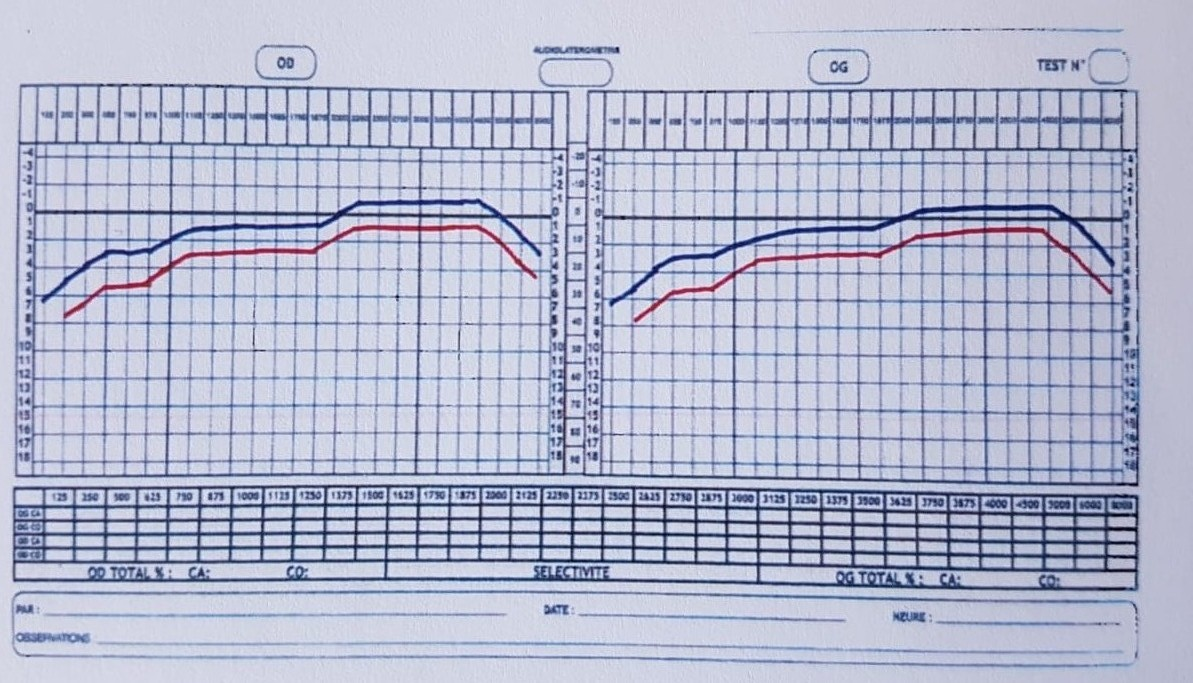
\includegraphics[width=0.7\linewidth]{images/courbeideale.jpg}
	\caption{Courbe idéale}
	\label{fig:courbeideale}
      \end{figure}

      
Sur le plan de la physique pure, elle indique les réponses de l'oreille
lorsque celle-ci fonctionne bien. Elle répond en fait à la courbe
de Wegel dite ``courbe en citron", inversée.\footnote{%
		Voir l'annexe \ref{acoustique} p. \pageref{acoustique}
		 pour cette partie technique.}.

               

L'acquisition de cette courbe idéale correspond à l'\textsl{harmonisation}
du jeu de deux muscles de l'oreille moyenne. Ce jeu
permet de régler en permanence la pression interne au niveau du
labyrinthe.
Lorsque l'interprétation des informations transmises à l'oreille est
erronée, il s'agit donc  de
distorsions d'écoute, déjà citées plus haut. Cette distorsion est liée au dysfonctionnement
de ces deux muscles de l'oreille moyenne dont le rôle est de permettre l'arrivée
harmonieuse du son dans l'oreille interne, puis au cerveau. Car, lorsque
le message sensoriel est altéré, le cerveau se protège en déclenchant
des mécanismes d'inhibition de l'écoute. On naît
avec ce potentiel mais celui-ci s'altère parfois avec les difficultés
de la vie et on introduit des distorsions
pour se défendre contre certaines agressions du monde extérieur. 

Sur le plan du test d'écoute, on remarquera
alors des distorsions, des manques par rapport à la courbe dite 
idéale.
Et lorsqu'il n'y a pas de distorsions, on parle d'harmonie. L'harmonie
est la régulation des émotions, l'équilibre entre son écoute
intérieure et extérieure. On la visualisera sous la forme de
courbes continues et parallèles.

%\enquote{\emph{L'oreille a un psychisme\autocite[{tomatis:loreille}.}} 

Le test d'écoute et ses paramètres:(8.3.2)




  




 




  

